% !TEX root = ../C++Prime-Plus-Notes.tex
% !TeX encoding = UTF-8

\chapter{处理数据}

\section{简单变量}

\subsection{整型short,int,long和long long}

在不同的系统中,short,int,long,long long的长度可能都是不同的,C++对其的标准为:

\begin{itemize}
\item short至少16位
\item int至少与short一样长
\item long至少32位,且至少与int一样长
\item long long至少64位,且至少与long一样长
\end{itemize}

以下程序运行在\stress{CentOS} 7 64位机上

\begin{cpp}
#include <iostream>
#include <climits>

int main(int argc, char|*| argv[]) {
    std::cout << sizeof(int) << std::endl; // 4
    std::cout << INT_MAX << std::endl;     // 2147483647
    return 0;
}
\end{cpp}

climits中还定义了许多符号常量,都是limits.h的套壳,具体可以查看limits.h\footnote{linux下一般在\codeline{/usr/include/limits.h}}文件,\tref{table:climits}也给出了一些。

\begin{table}[!hbt]
\centering
\begin{tabular}{p{18em}|p{18em}}
\hline
\stress{符号常量} & \stress{表示} \\
\hline
CHAR\_BIT & char的位数 \\
\hline
CHAR\_MAX & char的最大值 \\
\hline
CHAR\_MIN & char的最小值 \\
\hline
SCHAR\_MAX & signed char 的最大值 \\
\hline
SCHAR\_MIN & signed char 的最小值 \\
\hline
UCHAR\_MAX & unsigned char的最大值 \\
\hline
SHRT\_MAX & short的最大值 \\
\hline
SHRT\_MIN & short的最小值 \\
\hline
USHRT\_MAX & unsigned short的最大值 \\
\hline
INT\_MAX & int的最大值 \\
\hline
INT\_MIN & int的最小值 \\
\hline
UNIT\_MAX & unsigned int的最大值 \\
\hline
LONG\_MAX & long的最大值 \\
\hline
LONG\_MIN & long的最小值 \\
\hline
ULONG\_MAX & unsigned long的最大值 \\
\hline
LLONG\_MAX & long long的最大值 \\
\hline
LLONG\_MIN & long long的最小值 \\
\hline
ULLONG\_MAX & unsigned long long的最大值 \\
\hline
\end{tabular}
\caption{climits中的符号常量}
\label{table:climits}
\end{table}

\addtocounter{subsection}{4}

\subsection{整型字面值}

表示不同进制数的前缀,对于字符常量用\thinspace\fira{\mybackslash}\thinspace 代替\thinspace\fira{0}\thinspace:

\begin{itemize}
\item 二进制以\thinspace\fira{0b}\thinspace 开头
\item 八进制以\thinspace\fira{0}\thinspace 开头
\item 十六进制以\thinspace\fira{0x}\thinspace 开头
\end{itemize}

\subsection{C++如何确定常量的类型}

放在数字常量后面的字母用于表示类型,整数后面的l或L表示该整数为long常量,u或U后缀表示unsigned int常量,ul(不区分顺序和大小写)表示unsigned long常量,在C++11标准中,新加入了一些表示数字类型的后缀,具体见\tref{table:Numeric suffix}。

\begin{table}[!hbt]
\centering
\begin{tabular}{p{18em}|p{18em}}
\hline
\stress{后缀字母\footnotemark} & \stress{类型} \\
\hline
u & 表示unsigned int类型 \\
\hline
l & 表示long类型或long double 类型 \\
\hline
ll & 表示long long 类型 \\
\hline
ul & 表示unsigned long 类型 \\
\hline
ull & 表示 unsigned long long 类型 \\
\hline
f & 表示f\/loat 类型\\
\hline
\end{tabular}
\caption{数值后缀代表的类型}
\label{table:Numeric suffix}
\end{table}
\footnotetext{{不区分顺序和大小写}}

\subsection{char类型:字符和小整数}

论\codeline{\mybackslash n}和\codeline{endl}的区别\footnote{具体可以查看\thinspace\href{https://www.cnblogs.com/XqwKen/p/4564318.html}{endl与\thinspace\mybackslash n的区别}这篇文章}:\mybackslash n仅代表换行的转义字符,endl除了代表换行,还紧跟着清出缓冲槽。

cout的意思是console-output:控制台输出,就拿\codeline{cout << "Hello World!" <<\ }\\ \codeline{endl;}来说,cout代表后面的内容输出到控制台的一个缓冲槽,而不是控制台,当遇到endl或者其他f\/lush之类的命令或函数时,缓冲槽里的内容会按照顺序输出到控制台,再由控制台进行转义字符的识别打印。所以当你输入\codeline{cout << "Hello World!" << "\mybackslash n";}时,其实就相当于输入\codeline{cout << "Hello World!" << "\mybackslash n" <<  f\/lush;},程序会自动刷新输出流,所以只要你程序不炸,用\thinspace\mybackslash n比endl会快一点(不刷新输出流会快那么一点吧),但你如果程序够大并且明确要刷新输出流,就用endl吧。\dpar

C++支持直接输入\thinspace\href{https://home.unicode.org/}{\concept{Unicode}}\thinspace 码点,通用字符名可以以\codeline{\mybackslash u}或\codeline{\mybackslash U}打头,\mybackslash u后面跟的是4个十六进制位,\mybackslash U后面跟的是8个十六进制位,这里参见C++ prime plus英文版987页[There are two forms of UCN sequences. The first is \mybackslash u hexquad , where hexquad is a sequence of four hexadecimal digits; \mybackslash u00F6 is an example. The second is \mybackslash U hexquadhexquad ; \mybackslash U0000AC01 is an example. Because each hexadecimal digit corresponds to four bits, the \mybackslash u form can be used for codes representable by a 16-bit integer, and the \mybackslash U form can be used for codes representable by a 32-bit integer.],中文译版在第52页写的是8个十六进制位和16个十六进制位,应该是写错了。

\begin{cpp}
#include <iostream>
#include <string>

int main(int argc, char|*| argv[]) {
    std::string str = "\u2660\u2663\u2665\u2666";
    std::cout << str << std::endl; // ♠♣♥♦
    return 0;
}
\end{cpp}

一个char型占1个字节,也就是2个十六进制位,一般用来存放ASCII或者扩展的ACSII,C++内部还有一个内建的\codeline{wcha\_t}类型,在CentOS 7平台上测试其占4个字节,也就是8个十六进制位,可见其底层类型应该是unsigned int,在另外一些系统中其底层类型可能为unsigned short。如果你要用wcha\_t类型,由于cin和cout都将输入和输出都视为char流,不适合用来处理wcha\_t类型,iostream头文件的最新版中有\codeline{wcin}和\codeline{wcout}工具专门用来处理wcha\_t类型。另外,在一个字符常量前加L可以将其声明为宽字符常量,字符串也是一样。

\begin{cpp}
#include <iostream>

int main(int argc, char|*| argv[]) {
    wchar_t ch = L'\u262F';
    std::cout << sizeof(L'\u262F') << std::endl; // 4
    std::cout << ch << std::endl; // 9775
    std::wcout << ch << std::endl; // \
    return 0;
}
\end{cpp}

在这里我用的字符是U+262F[☯],可以看到宽字符常量占4个字节,cout输出流将其视为4个1字节的字符常量(即0x0000262F),转换成十进制时会忽略前面的0,输出便是9775,这里wcout的输出就是ACSII码的第97个,也就是\mybackslash ,想让wcout的输出正确的Unicode字符相当复杂\footnote{具体可以查看\thinspace\href{https://www.cnblogs.com/zyl910/archive/2013/01/20/wchar_crtbug_01.html}{cout,wcout无法正常输出中文字符问题的深入调查}这篇文章},而且不同的编译器实现也都不一样(虽然C++标准制定的很好,那有人不遵守咋办嘛)。

Unicode到目前为止已经定义了17个平面,除了第一个基本平面(简称BMP\fref{figure:Unicode BMP},其码点从U+0000到U+FFFF)用一个wcha\_t型存就会浪费两个字节,其他16个辅助平面(其码点从U+010000到U+10FFFD)用一个wcha\_t型刚好存下,如果你的程序用到了非常多的国际字符,用wcha\_t型可能就会存在空间浪费的情况(这里谈一下UTF-8吧,我觉得UTF-8流行的原因就是因为它兼顾了效率和容量,首先它实现了Unicode中的所有码点,其次它的变长编码保证了对于高频字符存储空间没有浪费,大概就像哈夫曼编码(Huffman Coding)一样吧),C++11中新增了\codeline{char16\_t}和\codeline{char32\_t}类型,这两种类型都是无符号的,其中前者长16位,后者长32位。C++11标准使用前缀u表示char16\_t类型字符常量和字符串常量(例如u\leftqm\mybackslash u262F\rightqm),用前缀U表示char32\_t类型字符常量和字符串常量(例如U\leftqm\mybackslash U0001F602\rightqm),这两个类型应该和UTF-16编码和UTF-32编码相对应吧,但鉴于UTF-16是变长编码(好吧,就是两个字节根本不够用),\sout{我也不知道有没有关系}(在\thinspace\href{https://github.com/google/styleguide}{Google风格指南}里明确了它们用于非UTF-8文本,但不推荐你使用这两个类型)。

\begin{figure}[!hbt]
\centering
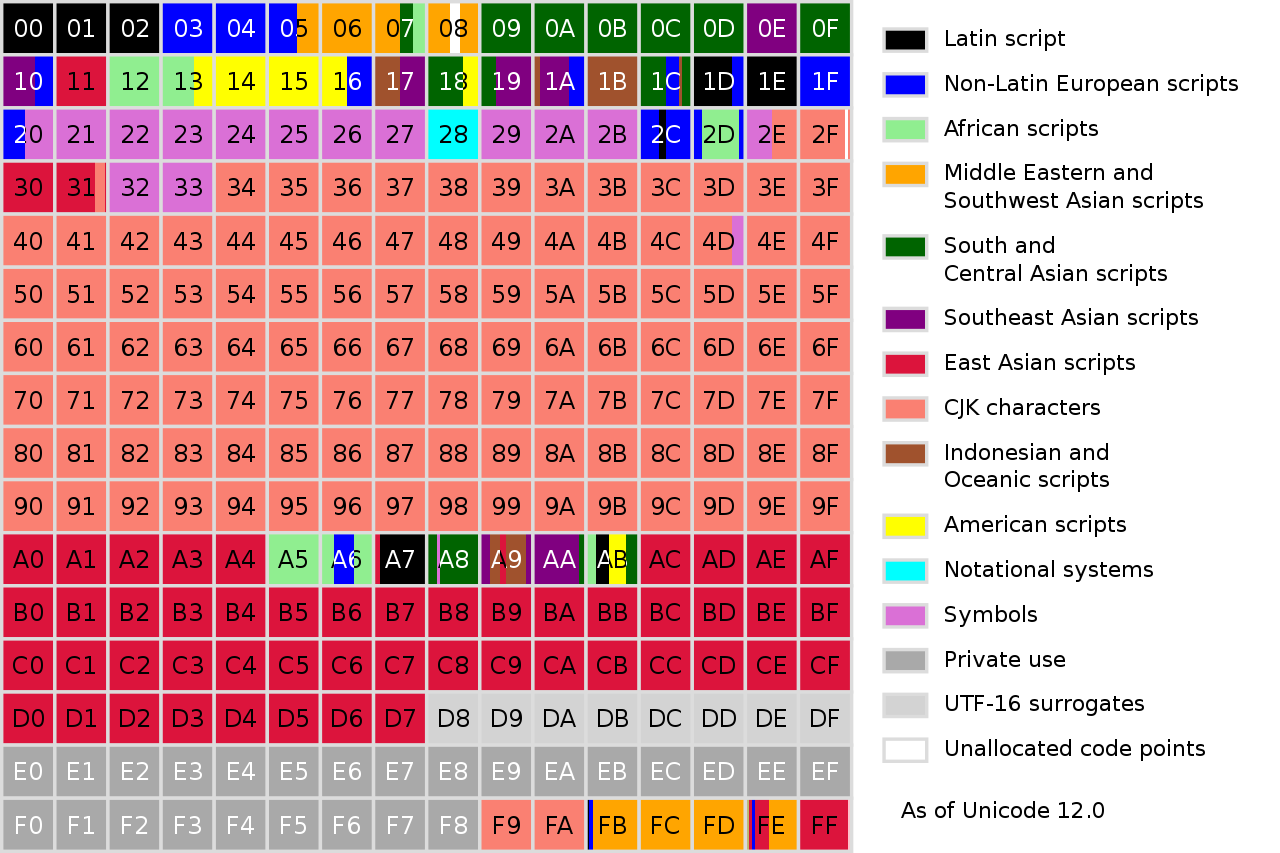
\includegraphics[scale=0.3]{./Figures/Unicode BMP}
\caption{A graphical representation of Unicode\rightqm s Basic Multilingual Plane(BMP)}
\label{figure:Unicode BMP}
\end{figure}

搞了怎么多类型,有char,wcha\_t,char16\_t,char32\_t,而且有的用起来还十分的不方便(这里提名wcin和wcout),所以在上面那个程序里用的是\codeline{std::string},其实C++标准库已经帮我们实现好了string类,而且它相比\codeline{char* []}非常智能(到后面\codeline{std::cin.get()}的时候就会知道),如果你不是一定要用char,用string会方便地多。

\section{const限定符}

C++中\codeline{\#define}和\codeline{const}的区别:

\begin{itemize}
\item 用\codeline{\#def\/ine MAX 255}定义的常量是没有类型的,所给出的是一个数,编译器只是把所定义的常量值与所定义的常量的名字联系起来,\#def\/ine所定义的宏变量在预处理的时候进行替换,在程序中使用到该常量的地方都要进行拷贝替换。用\codeline{const f\/loat MAX = }\\ \codeline{255}定义的常量有类型名字,存放在内存的静态区域中,在程序运行过程中const变量只有一个拷贝,而\#def\/ine 所定义的宏变量却有多个拷贝,所以宏定义在程序运行过程中所消耗的内存要比const变量的大得多
\item 用\#def\/ine定义的常量是不可以用指针变量去指向的,用const定义的常量是可以用指针去指向该常量的地址的
\item 用\#def\/ine可以定义一些简单的函数,const是不可以定义函数的
\end{itemize}

在编译时,编译器通常不为const常量分配存储空间,而是将它们保存在符号表中,这使得它成为一个编译期间的常量,没有了存储与读内存的操作,使得它的效率也很高。宏定义的作用范围仅限于当前文件,且只作替换,不做计算,不做表达式求解。默认状态下,const对象只在文件内有效,当多个文件中出现了同名的const变量时,等同于在不同文件中分别定义了独立的变量。如果想在多个文件之间共享const对象,必须在变量定义之前添加extern关键字(在声明和定义时都要加)。const有数据类型,编译时会进行类型检查,而\#def\/ine无类型,也不进行类型安全检查,可能会产生意想不到的错误,因此如果你不是明确知道自己在干什么,尽量只使用const常量而不使用宏常量。

\section{浮点数}

\addtocounter{subsection}{1}

\subsection{浮点类型}

先说一下计算机中浮点数的存法吧,IEEE-754\cite{IEEE754}规定,对于32位的浮点数,最高的1位是符号位S,接着的8位是指数E,剩下的23位为有效数字M,就拿\fref{figure:Float}中的这个浮点数来

\begin{figure}[!hbt]
\centering
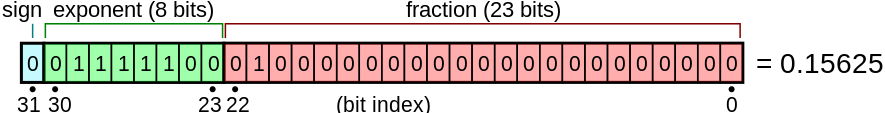
\includegraphics[scale=0.4]{./Figures/Float}
\caption{0b0111110001000000000000000000000}
\label{figure:Float}
\end{figure}

\noindent 说,其真值的计算公式为$X=(-1)^S*M*2^{E-127}$,其中M为尾数,127称为偏移量,这只是一个最普通的偏移类型的浮点数,IEEE-754还规定了很多类型的浮点数,在这里就不一一赘述了。还有就是我们生活中的很多十进制小数转换成浮点数的时候都会丢失精度,32位的丢失的多一点,64位的丢失的少一点罢了,就拿0.7这个数来说,十进制小数转换成二进制的规则是:小数点前的部分\stress{除2取余逆序排列}小数点后的部分\stress{乘2取整顺序排列},所以0.7转换成二进制小数就是0.101100110\dots,你拿多少位的浮点数存都会有丢失精度的情况,只不过是丢失的多少罢了。

\section{C++算数运算符}

\addtocounter{subsection}{3}

\subsection{类型转换}

C++11对于类型转换有一个表,编译器会查这个表进行类型转换:

\begin{enumerate}
\item 如果有一个操作数的类型是long double,则将另一个操作数转换为long double
\item 否则,如果有一个操作数的类型是double,则将另一个操作数转换为double
\item 否则,如果有一个操作数的类型是f\/loat,则将另一个操作数转换为f\/loat
\item 否则,说明操作数都是整型,因此执行整型提升
\item 在这种情况下,如果两个操作数都是有符号或无符号的,且其中一个操作数的级别比另一个低,则转换为级别高的类型
\item 如果一个操作数是有符号的,另一个操作数是无符号的,且无符号操作数的级别比有符号操作数高,则将有符号操作数转换为无符号操作数所属的类型
\item 否则。如果有符号类型可表示无符号类型的所有可能取值,则将无符号操作数转换为有符号操作数所属的类型
\item 否则,将两个操作数都转换为有符号类型的无符号版本
\end{enumerate}\mbox{}

上述都是在表达式中的类型转换,如果你在赋值时将一个值赋给一个取值范围更小的值,可能就会出现潜在的数值转换问题,见\tref{table:Conversion}。

\begin{table}[!hbt]
\centering
\begin{tabular}{p{18em}|p{18em}}
\hline
\stress{转换} & \stress{潜在的问题} \\
\hline
将较大的浮点类型转换为较小的浮点类型,如将double转换为f\/loat & 精度(有效位数)降低,值可能超出目标类型的取值范围,在这种情况下,结果将是不确定的 \\
\hline
将浮点类型转换为整型 & 小数部分丢失,值可能超出目标类型的范围,在这种情况下,结果将是不确定的 \\
\hline
将较大的整型转换为较小的整型,如将long转换问short & 原来的值可能超出目标类型的取值范围,通常只复制右边的字节 \\
\hline
\end{tabular}
\caption{潜在的数值转换问题}
\label{table:Conversion}
\end{table}
